% Graphic for TeX using PGF
% Title: C:\Users\Nicolas Chicaiza\Sourcetree\Metodología de la Investigación\Enfoque Marco Lógico\Esquemas\Árbol de Objetivos\arbolObjetivos.dia
% Creator: Dia v0.97.2
% CreationDate: Mon May 03 09:04:47 2021
% For: Nicolas Chicaiza
% \usepackage{tikz}
% The following commands are not supported in PSTricks at present
% We define them conditionally, so when they are implemented,
% this pgf file will use them.
\ifx\du\undefined
  \newlength{\du}
\fi
\setlength{\du}{15\unitlength}
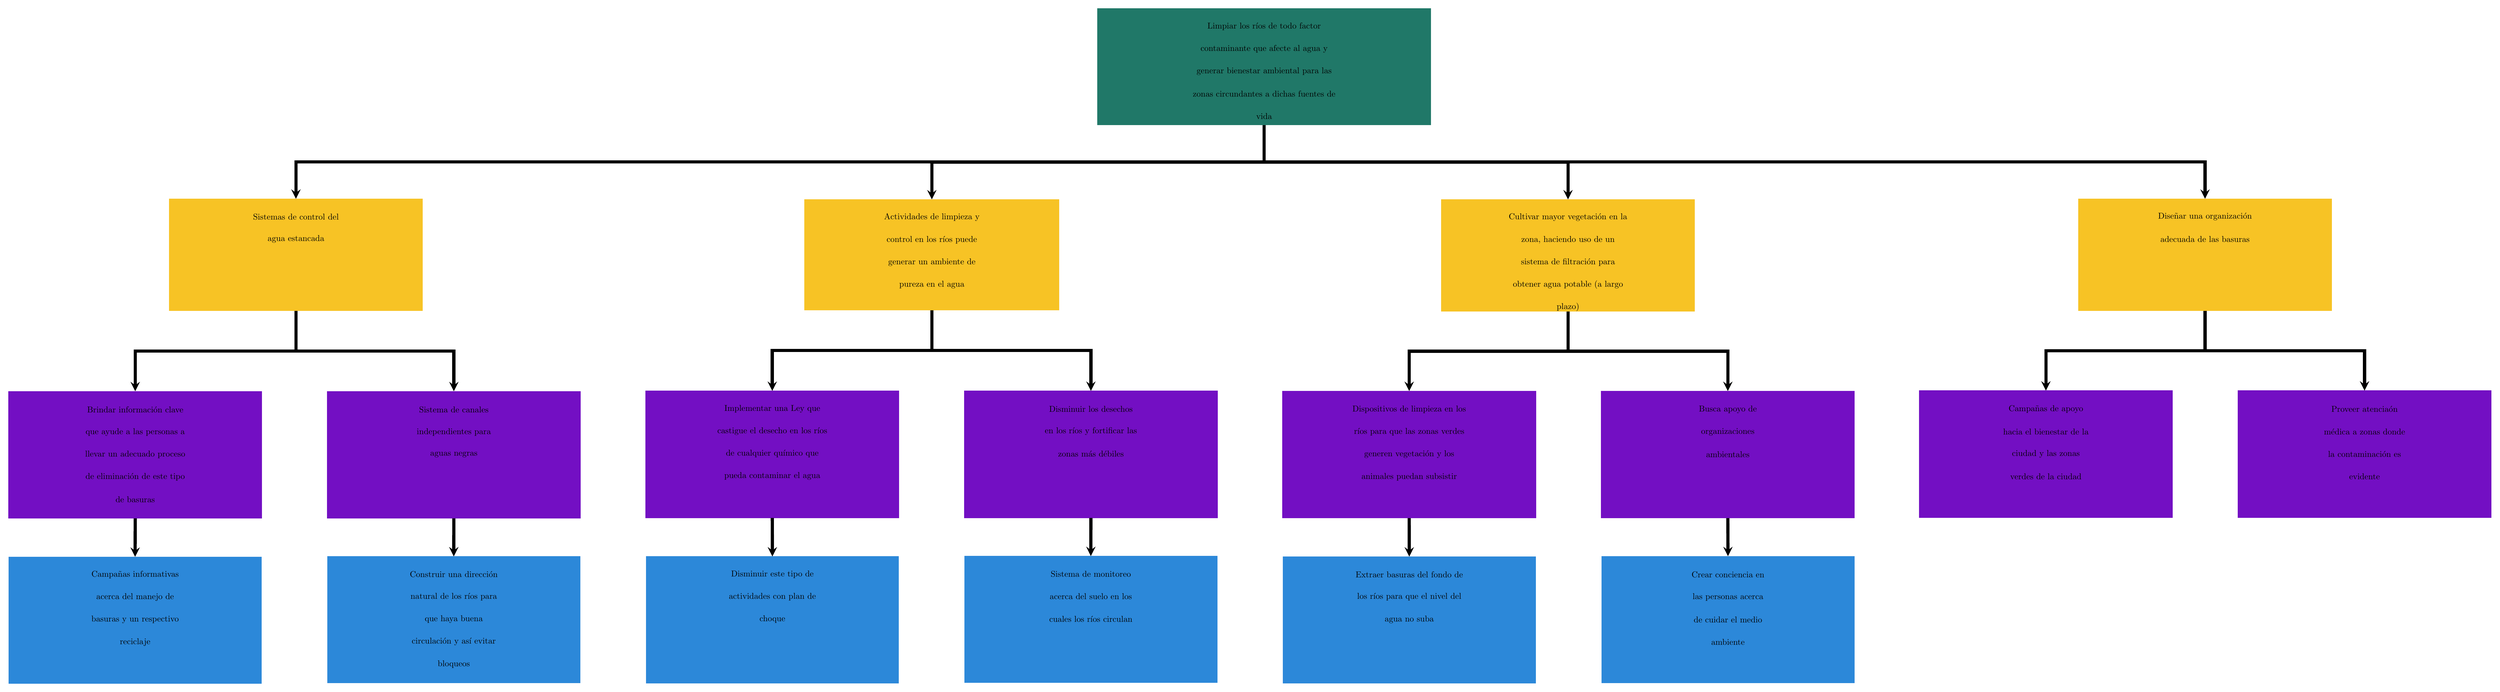
\begin{tikzpicture}
\pgftransformxscale{1.000000}
\pgftransformyscale{-1.000000}
\definecolor{dialinecolor}{rgb}{0.000000, 0.000000, 0.000000}
\pgfsetstrokecolor{dialinecolor}
\definecolor{dialinecolor}{rgb}{1.000000, 1.000000, 1.000000}
\pgfsetfillcolor{dialinecolor}
\pgfsetlinewidth{0.000000\du}
\pgfsetdash{}{0pt}
\pgfsetdash{}{0pt}
\pgfsetmiterjoin
\definecolor{dialinecolor}{rgb}{0.125490, 0.470588, 0.407843}
\pgfsetfillcolor{dialinecolor}
\fill (32.989121\du,12.050000\du)--(32.989121\du,21.200000\du)--(59.189121\du,21.200000\du)--(59.189121\du,12.050000\du)--cycle;
\definecolor{dialinecolor}{rgb}{0.125490, 0.470588, 0.407843}
\pgfsetstrokecolor{dialinecolor}
\draw (32.989121\du,12.050000\du)--(32.989121\du,21.200000\du)--(59.189121\du,21.200000\du)--(59.189121\du,12.050000\du)--cycle;
% setfont left to latex
\definecolor{dialinecolor}{rgb}{1.000000, 1.000000, 1.000000}
\pgfsetstrokecolor{dialinecolor}
\node at (46.089121\du,13.460000\du){Limpiar los ríos de todo factor};
% setfont left to latex
\definecolor{dialinecolor}{rgb}{1.000000, 1.000000, 1.000000}
\pgfsetstrokecolor{dialinecolor}
\node at (46.089121\du,15.223889\du){contaminante que afecte al agua y};
% setfont left to latex
\definecolor{dialinecolor}{rgb}{1.000000, 1.000000, 1.000000}
\pgfsetstrokecolor{dialinecolor}
\node at (46.089121\du,16.987778\du){generar bienestar ambiental para las};
% setfont left to latex
\definecolor{dialinecolor}{rgb}{1.000000, 1.000000, 1.000000}
\pgfsetstrokecolor{dialinecolor}
\node at (46.089121\du,18.751667\du){zonas circundantes a dichas fuentes de};
% setfont left to latex
\definecolor{dialinecolor}{rgb}{1.000000, 1.000000, 1.000000}
\pgfsetstrokecolor{dialinecolor}
\node at (46.089121\du,20.515556\du){vida};
\pgfsetlinewidth{0.000000\du}
\pgfsetdash{}{0pt}
\pgfsetdash{}{0pt}
\pgfsetmiterjoin
\definecolor{dialinecolor}{rgb}{0.968627, 0.764706, 0.145098}
\pgfsetfillcolor{dialinecolor}
\fill (9.994752\du,27.050000\du)--(9.994752\du,35.750000\du)--(29.994752\du,35.750000\du)--(29.994752\du,27.050000\du)--cycle;
\definecolor{dialinecolor}{rgb}{0.968627, 0.764706, 0.145098}
\pgfsetstrokecolor{dialinecolor}
\draw (9.994752\du,27.050000\du)--(9.994752\du,35.750000\du)--(29.994752\du,35.750000\du)--(29.994752\du,27.050000\du)--cycle;
% setfont left to latex
\definecolor{dialinecolor}{rgb}{1.000000, 1.000000, 1.000000}
\pgfsetstrokecolor{dialinecolor}
\node at (19.994752\du,28.460000\du){Actividades de limpieza y};
% setfont left to latex
\definecolor{dialinecolor}{rgb}{1.000000, 1.000000, 1.000000}
\pgfsetstrokecolor{dialinecolor}
\node at (19.994752\du,30.223889\du){control en los ríos puede};
% setfont left to latex
\definecolor{dialinecolor}{rgb}{1.000000, 1.000000, 1.000000}
\pgfsetstrokecolor{dialinecolor}
\node at (19.994752\du,31.987778\du){generar un ambiente de};
% setfont left to latex
\definecolor{dialinecolor}{rgb}{1.000000, 1.000000, 1.000000}
\pgfsetstrokecolor{dialinecolor}
\node at (19.994752\du,33.751667\du){pureza en el agua};
\pgfsetlinewidth{0.250000\du}
\pgfsetdash{}{0pt}
\pgfsetdash{}{0pt}
\pgfsetmiterjoin
\pgfsetbuttcap
{
\definecolor{dialinecolor}{rgb}{0.000000, 0.000000, 0.000000}
\pgfsetfillcolor{dialinecolor}
% was here!!!
\pgfsetarrowsend{stealth}
{\pgfsetcornersarced{\pgfpoint{0.000000\du}{0.000000\du}}\definecolor{dialinecolor}{rgb}{0.000000, 0.000000, 0.000000}
\pgfsetstrokecolor{dialinecolor}
\draw (46.089121\du,21.200000\du)--(46.089121\du,24.114842\du)--(19.994752\du,24.114842\du)--(19.994752\du,27.050000\du);
}}
\pgfsetlinewidth{0.000000\du}
\pgfsetdash{}{0pt}
\pgfsetdash{}{0pt}
\pgfsetmiterjoin
\definecolor{dialinecolor}{rgb}{0.968627, 0.764706, 0.145098}
\pgfsetfillcolor{dialinecolor}
\fill (60.005205\du,27.050000\du)--(60.005205\du,35.850000\du)--(79.905205\du,35.850000\du)--(79.905205\du,27.050000\du)--cycle;
\definecolor{dialinecolor}{rgb}{0.968627, 0.764706, 0.145098}
\pgfsetstrokecolor{dialinecolor}
\draw (60.005205\du,27.050000\du)--(60.005205\du,35.850000\du)--(79.905205\du,35.850000\du)--(79.905205\du,27.050000\du)--cycle;
% setfont left to latex
\definecolor{dialinecolor}{rgb}{1.000000, 1.000000, 1.000000}
\pgfsetstrokecolor{dialinecolor}
\node at (69.955205\du,28.460000\du){Cultivar mayor vegetación en la};
% setfont left to latex
\definecolor{dialinecolor}{rgb}{1.000000, 1.000000, 1.000000}
\pgfsetstrokecolor{dialinecolor}
\node at (69.955205\du,30.223889\du){zona, haciendo uso de un};
% setfont left to latex
\definecolor{dialinecolor}{rgb}{1.000000, 1.000000, 1.000000}
\pgfsetstrokecolor{dialinecolor}
\node at (69.955205\du,31.987778\du){sistema de filtración para};
% setfont left to latex
\definecolor{dialinecolor}{rgb}{1.000000, 1.000000, 1.000000}
\pgfsetstrokecolor{dialinecolor}
\node at (69.955205\du,33.751667\du){obtener agua potable (a largo};
% setfont left to latex
\definecolor{dialinecolor}{rgb}{1.000000, 1.000000, 1.000000}
\pgfsetstrokecolor{dialinecolor}
\node at (69.955205\du,35.515556\du){plazo)};
\pgfsetlinewidth{0.250000\du}
\pgfsetdash{}{0pt}
\pgfsetdash{}{0pt}
\pgfsetmiterjoin
\pgfsetbuttcap
{
\definecolor{dialinecolor}{rgb}{0.000000, 0.000000, 0.000000}
\pgfsetfillcolor{dialinecolor}
% was here!!!
\pgfsetarrowsend{stealth}
{\pgfsetcornersarced{\pgfpoint{0.000000\du}{0.000000\du}}\definecolor{dialinecolor}{rgb}{0.000000, 0.000000, 0.000000}
\pgfsetstrokecolor{dialinecolor}
\draw (46.089121\du,21.200000\du)--(46.089121\du,24.114842\du)--(69.955205\du,24.114842\du)--(69.955205\du,27.050000\du);
}}
\pgfsetlinewidth{0.000000\du}
\pgfsetdash{}{0pt}
\pgfsetdash{}{0pt}
\pgfsetmiterjoin
\definecolor{dialinecolor}{rgb}{0.968627, 0.764706, 0.145098}
\pgfsetfillcolor{dialinecolor}
\fill (-39.894516\du,27.000000\du)--(-39.894516\du,35.800000\du)--(-19.994516\du,35.800000\du)--(-19.994516\du,27.000000\du)--cycle;
\definecolor{dialinecolor}{rgb}{0.968627, 0.764706, 0.145098}
\pgfsetstrokecolor{dialinecolor}
\draw (-39.894516\du,27.000000\du)--(-39.894516\du,35.800000\du)--(-19.994516\du,35.800000\du)--(-19.994516\du,27.000000\du)--cycle;
% setfont left to latex
\definecolor{dialinecolor}{rgb}{1.000000, 1.000000, 1.000000}
\pgfsetstrokecolor{dialinecolor}
\node at (-29.944516\du,28.410000\du){Sistemas de control del};
% setfont left to latex
\definecolor{dialinecolor}{rgb}{1.000000, 1.000000, 1.000000}
\pgfsetstrokecolor{dialinecolor}
\node at (-29.944516\du,30.173889\du){agua estancada};
\pgfsetlinewidth{0.250000\du}
\pgfsetdash{}{0pt}
\pgfsetdash{}{0pt}
\pgfsetmiterjoin
\pgfsetbuttcap
{
\definecolor{dialinecolor}{rgb}{0.000000, 0.000000, 0.000000}
\pgfsetfillcolor{dialinecolor}
% was here!!!
\pgfsetarrowsend{stealth}
{\pgfsetcornersarced{\pgfpoint{0.000000\du}{0.000000\du}}\definecolor{dialinecolor}{rgb}{0.000000, 0.000000, 0.000000}
\pgfsetstrokecolor{dialinecolor}
\draw (46.089121\du,21.200000\du)--(46.089121\du,24.100000\du)--(-29.944516\du,24.100000\du)--(-29.944516\du,27.000000\du);
}}
\pgfsetlinewidth{0.000000\du}
\pgfsetdash{}{0pt}
\pgfsetdash{}{0pt}
\pgfsetmiterjoin
\definecolor{dialinecolor}{rgb}{0.968627, 0.764706, 0.145098}
\pgfsetfillcolor{dialinecolor}
\fill (110.030896\du,27.000000\du)--(110.030896\du,35.800000\du)--(129.930896\du,35.800000\du)--(129.930896\du,27.000000\du)--cycle;
\definecolor{dialinecolor}{rgb}{0.968627, 0.764706, 0.145098}
\pgfsetstrokecolor{dialinecolor}
\draw (110.030896\du,27.000000\du)--(110.030896\du,35.800000\du)--(129.930896\du,35.800000\du)--(129.930896\du,27.000000\du)--cycle;
% setfont left to latex
\definecolor{dialinecolor}{rgb}{1.000000, 1.000000, 1.000000}
\pgfsetstrokecolor{dialinecolor}
\node at (119.980896\du,28.410000\du){Diseñar una organización};
% setfont left to latex
\definecolor{dialinecolor}{rgb}{1.000000, 1.000000, 1.000000}
\pgfsetstrokecolor{dialinecolor}
\node at (119.980896\du,30.173889\du){adecuada de las basuras};
\pgfsetlinewidth{0.250000\du}
\pgfsetdash{}{0pt}
\pgfsetdash{}{0pt}
\pgfsetmiterjoin
\pgfsetbuttcap
{
\definecolor{dialinecolor}{rgb}{0.000000, 0.000000, 0.000000}
\pgfsetfillcolor{dialinecolor}
% was here!!!
\pgfsetarrowsend{stealth}
{\pgfsetcornersarced{\pgfpoint{0.000000\du}{0.000000\du}}\definecolor{dialinecolor}{rgb}{0.000000, 0.000000, 0.000000}
\pgfsetstrokecolor{dialinecolor}
\draw (46.089121\du,21.200000\du)--(46.089121\du,24.100000\du)--(119.980896\du,24.100000\du)--(119.980896\du,27.000000\du);
}}
\pgfsetlinewidth{0.000000\du}
\pgfsetdash{}{0pt}
\pgfsetdash{}{0pt}
\pgfsetmiterjoin
\definecolor{dialinecolor}{rgb}{0.450980, 0.058824, 0.764706}
\pgfsetfillcolor{dialinecolor}
\fill (-2.488883\du,42.095259\du)--(-2.488883\du,52.080925\du)--(17.417607\du,52.080925\du)--(17.417607\du,42.095259\du)--cycle;
\definecolor{dialinecolor}{rgb}{0.450980, 0.058824, 0.764706}
\pgfsetstrokecolor{dialinecolor}
\draw (-2.488883\du,42.095259\du)--(-2.488883\du,52.080925\du)--(17.417607\du,52.080925\du)--(17.417607\du,42.095259\du)--cycle;
% setfont left to latex
\definecolor{dialinecolor}{rgb}{1.000000, 1.000000, 1.000000}
\pgfsetstrokecolor{dialinecolor}
\node at (7.464362\du,43.505259\du){Implementar una Ley que};
% setfont left to latex
\definecolor{dialinecolor}{rgb}{1.000000, 1.000000, 1.000000}
\pgfsetstrokecolor{dialinecolor}
\node at (7.464362\du,45.269148\du){ castigue el desecho en los ríos};
% setfont left to latex
\definecolor{dialinecolor}{rgb}{1.000000, 1.000000, 1.000000}
\pgfsetstrokecolor{dialinecolor}
\node at (7.464362\du,47.033037\du){de cualquier químico que};
% setfont left to latex
\definecolor{dialinecolor}{rgb}{1.000000, 1.000000, 1.000000}
\pgfsetstrokecolor{dialinecolor}
\node at (7.464362\du,48.796926\du){pueda contaminar el agua};
\pgfsetlinewidth{0.250000\du}
\pgfsetdash{}{0pt}
\pgfsetdash{}{0pt}
\pgfsetmiterjoin
\pgfsetbuttcap
{
\definecolor{dialinecolor}{rgb}{0.000000, 0.000000, 0.000000}
\pgfsetfillcolor{dialinecolor}
% was here!!!
\pgfsetarrowsend{stealth}
{\pgfsetcornersarced{\pgfpoint{0.000000\du}{0.000000\du}}\definecolor{dialinecolor}{rgb}{0.000000, 0.000000, 0.000000}
\pgfsetstrokecolor{dialinecolor}
\draw (19.994752\du,35.750000\du)--(19.994752\du,38.922630\du)--(7.464362\du,38.922630\du)--(7.464362\du,42.095259\du);
}}
\pgfsetlinewidth{0.000000\du}
\pgfsetdash{}{0pt}
\pgfsetdash{}{0pt}
\pgfsetmiterjoin
\definecolor{dialinecolor}{rgb}{0.450980, 0.058824, 0.764706}
\pgfsetfillcolor{dialinecolor}
\fill (22.533640\du,42.095259\du)--(22.533640\du,52.080925\du)--(42.440130\du,52.080925\du)--(42.440130\du,42.095259\du)--cycle;
\definecolor{dialinecolor}{rgb}{0.450980, 0.058824, 0.764706}
\pgfsetstrokecolor{dialinecolor}
\draw (22.533640\du,42.095259\du)--(22.533640\du,52.080925\du)--(42.440130\du,52.080925\du)--(42.440130\du,42.095259\du)--cycle;
% setfont left to latex
\definecolor{dialinecolor}{rgb}{1.000000, 1.000000, 1.000000}
\pgfsetstrokecolor{dialinecolor}
\node at (32.486885\du,43.505259\du){Disminuir los desechos};
% setfont left to latex
\definecolor{dialinecolor}{rgb}{1.000000, 1.000000, 1.000000}
\pgfsetstrokecolor{dialinecolor}
\node at (32.486885\du,45.269148\du){en los ríos y fortificar las};
% setfont left to latex
\definecolor{dialinecolor}{rgb}{1.000000, 1.000000, 1.000000}
\pgfsetstrokecolor{dialinecolor}
\node at (32.486885\du,47.033037\du){zonas más débiles};
\pgfsetlinewidth{0.250000\du}
\pgfsetdash{}{0pt}
\pgfsetdash{}{0pt}
\pgfsetmiterjoin
\pgfsetbuttcap
{
\definecolor{dialinecolor}{rgb}{0.000000, 0.000000, 0.000000}
\pgfsetfillcolor{dialinecolor}
% was here!!!
\pgfsetarrowsend{stealth}
{\pgfsetcornersarced{\pgfpoint{0.000000\du}{0.000000\du}}\definecolor{dialinecolor}{rgb}{0.000000, 0.000000, 0.000000}
\pgfsetstrokecolor{dialinecolor}
\draw (19.994752\du,35.750000\du)--(19.994752\du,38.922630\du)--(32.486885\du,38.922630\du)--(32.486885\du,42.095259\du);
}}
\pgfsetlinewidth{0.000000\du}
\pgfsetdash{}{0pt}
\pgfsetdash{}{0pt}
\pgfsetmiterjoin
\definecolor{dialinecolor}{rgb}{0.172549, 0.533333, 0.850980}
\pgfsetfillcolor{dialinecolor}
\fill (-2.451739\du,55.103962\du)--(-2.451739\du,65.058081\du)--(17.397084\du,65.058081\du)--(17.397084\du,55.103962\du)--cycle;
\definecolor{dialinecolor}{rgb}{0.172549, 0.533333, 0.850980}
\pgfsetstrokecolor{dialinecolor}
\draw (-2.451739\du,55.103962\du)--(-2.451739\du,65.058081\du)--(17.397084\du,65.058081\du)--(17.397084\du,55.103962\du)--cycle;
\pgfsetlinewidth{0.250000\du}
\pgfsetdash{}{0pt}
\pgfsetdash{}{0pt}
\pgfsetbuttcap
{
\definecolor{dialinecolor}{rgb}{0.000000, 0.000000, 0.000000}
\pgfsetfillcolor{dialinecolor}
% was here!!!
\pgfsetarrowsend{stealth}
\definecolor{dialinecolor}{rgb}{0.000000, 0.000000, 0.000000}
\pgfsetstrokecolor{dialinecolor}
\draw (7.464362\du,52.080925\du)--(7.472672\du,55.103962\du);
}
% setfont left to latex
\definecolor{dialinecolor}{rgb}{1.000000, 1.000000, 1.000000}
\pgfsetstrokecolor{dialinecolor}
\node at (7.472672\du,56.513962\du){Disminuir este tipo de};
% setfont left to latex
\definecolor{dialinecolor}{rgb}{1.000000, 1.000000, 1.000000}
\pgfsetstrokecolor{dialinecolor}
\node at (7.472672\du,58.277851\du){actividades con plan de};
% setfont left to latex
\definecolor{dialinecolor}{rgb}{1.000000, 1.000000, 1.000000}
\pgfsetstrokecolor{dialinecolor}
\node at (7.472672\du,60.041740\du){choque};
\pgfsetlinewidth{0.000000\du}
\pgfsetdash{}{0pt}
\pgfsetdash{}{0pt}
\pgfsetmiterjoin
\definecolor{dialinecolor}{rgb}{0.172549, 0.533333, 0.850980}
\pgfsetfillcolor{dialinecolor}
\fill (22.556693\du,55.072279\du)--(22.556693\du,65.026399\du)--(42.405516\du,65.026399\du)--(42.405516\du,55.072279\du)--cycle;
\definecolor{dialinecolor}{rgb}{0.172549, 0.533333, 0.850980}
\pgfsetstrokecolor{dialinecolor}
\draw (22.556693\du,55.072279\du)--(22.556693\du,65.026399\du)--(42.405516\du,65.026399\du)--(42.405516\du,55.072279\du)--cycle;
% setfont left to latex
\definecolor{dialinecolor}{rgb}{1.000000, 1.000000, 1.000000}
\pgfsetstrokecolor{dialinecolor}
\node at (32.481105\du,56.482279\du){Sistema de monitoreo};
% setfont left to latex
\definecolor{dialinecolor}{rgb}{1.000000, 1.000000, 1.000000}
\pgfsetstrokecolor{dialinecolor}
\node at (32.481105\du,58.246168\du){acerca del suelo en los};
% setfont left to latex
\definecolor{dialinecolor}{rgb}{1.000000, 1.000000, 1.000000}
\pgfsetstrokecolor{dialinecolor}
\node at (32.481105\du,60.010057\du){cuales los ríos circulan};
\pgfsetlinewidth{0.250000\du}
\pgfsetdash{}{0pt}
\pgfsetdash{}{0pt}
\pgfsetbuttcap
{
\definecolor{dialinecolor}{rgb}{0.000000, 0.000000, 0.000000}
\pgfsetfillcolor{dialinecolor}
% was here!!!
\pgfsetarrowsend{stealth}
\definecolor{dialinecolor}{rgb}{0.000000, 0.000000, 0.000000}
\pgfsetstrokecolor{dialinecolor}
\draw (32.486885\du,52.080925\du)--(32.481105\du,55.072279\du);
}
\pgfsetlinewidth{0.000000\du}
\pgfsetdash{}{0pt}
\pgfsetdash{}{0pt}
\pgfsetmiterjoin
\definecolor{dialinecolor}{rgb}{0.450980, 0.058824, 0.764706}
\pgfsetfillcolor{dialinecolor}
\fill (-52.519341\du,42.123175\du)--(-52.519341\du,52.108841\du)--(-32.612851\du,52.108841\du)--(-32.612851\du,42.123175\du)--cycle;
\definecolor{dialinecolor}{rgb}{0.450980, 0.058824, 0.764706}
\pgfsetstrokecolor{dialinecolor}
\draw (-52.519341\du,42.123175\du)--(-52.519341\du,52.108841\du)--(-32.612851\du,52.108841\du)--(-32.612851\du,42.123175\du)--cycle;
% setfont left to latex
\definecolor{dialinecolor}{rgb}{1.000000, 1.000000, 1.000000}
\pgfsetstrokecolor{dialinecolor}
\node at (-42.566096\du,43.575675\du){Brindar información clave};
% setfont left to latex
\definecolor{dialinecolor}{rgb}{1.000000, 1.000000, 1.000000}
\pgfsetstrokecolor{dialinecolor}
\node at (-42.566096\du,45.339564\du){que ayude a las personas a};
% setfont left to latex
\definecolor{dialinecolor}{rgb}{1.000000, 1.000000, 1.000000}
\pgfsetstrokecolor{dialinecolor}
\node at (-42.566096\du,47.103453\du){llevar un adecuado proceso};
% setfont left to latex
\definecolor{dialinecolor}{rgb}{1.000000, 1.000000, 1.000000}
\pgfsetstrokecolor{dialinecolor}
\node at (-42.566096\du,48.867342\du){de eliminación de este tipo};
% setfont left to latex
\definecolor{dialinecolor}{rgb}{1.000000, 1.000000, 1.000000}
\pgfsetstrokecolor{dialinecolor}
\node at (-42.566096\du,50.631231\du){de basuras};
\pgfsetlinewidth{0.250000\du}
\pgfsetdash{}{0pt}
\pgfsetdash{}{0pt}
\pgfsetmiterjoin
\pgfsetbuttcap
{
\definecolor{dialinecolor}{rgb}{0.000000, 0.000000, 0.000000}
\pgfsetfillcolor{dialinecolor}
% was here!!!
\pgfsetarrowsend{stealth}
{\pgfsetcornersarced{\pgfpoint{0.000000\du}{0.000000\du}}\definecolor{dialinecolor}{rgb}{0.000000, 0.000000, 0.000000}
\pgfsetstrokecolor{dialinecolor}
\draw (-29.944516\du,35.800000\du)--(-29.944516\du,38.961588\du)--(-42.566096\du,38.961588\du)--(-42.566096\du,42.123175\du);
}}
\pgfsetlinewidth{0.000000\du}
\pgfsetdash{}{0pt}
\pgfsetdash{}{0pt}
\pgfsetmiterjoin
\definecolor{dialinecolor}{rgb}{0.450980, 0.058824, 0.764706}
\pgfsetfillcolor{dialinecolor}
\fill (-27.496818\du,42.123175\du)--(-27.496818\du,52.108841\du)--(-7.590328\du,52.108841\du)--(-7.590328\du,42.123175\du)--cycle;
\definecolor{dialinecolor}{rgb}{0.450980, 0.058824, 0.764706}
\pgfsetstrokecolor{dialinecolor}
\draw (-27.496818\du,42.123175\du)--(-27.496818\du,52.108841\du)--(-7.590328\du,52.108841\du)--(-7.590328\du,42.123175\du)--cycle;
% setfont left to latex
\definecolor{dialinecolor}{rgb}{1.000000, 1.000000, 1.000000}
\pgfsetstrokecolor{dialinecolor}
\node at (-17.543573\du,43.575675\du){Sistema de canales};
% setfont left to latex
\definecolor{dialinecolor}{rgb}{1.000000, 1.000000, 1.000000}
\pgfsetstrokecolor{dialinecolor}
\node at (-17.543573\du,45.339564\du){independientes para};
% setfont left to latex
\definecolor{dialinecolor}{rgb}{1.000000, 1.000000, 1.000000}
\pgfsetstrokecolor{dialinecolor}
\node at (-17.543573\du,47.103453\du){aguas negras};
\pgfsetlinewidth{0.250000\du}
\pgfsetdash{}{0pt}
\pgfsetdash{}{0pt}
\pgfsetmiterjoin
\pgfsetbuttcap
{
\definecolor{dialinecolor}{rgb}{0.000000, 0.000000, 0.000000}
\pgfsetfillcolor{dialinecolor}
% was here!!!
\pgfsetarrowsend{stealth}
{\pgfsetcornersarced{\pgfpoint{0.000000\du}{0.000000\du}}\definecolor{dialinecolor}{rgb}{0.000000, 0.000000, 0.000000}
\pgfsetstrokecolor{dialinecolor}
\draw (-29.944516\du,35.800000\du)--(-29.944516\du,38.961588\du)--(-17.543573\du,38.961588\du)--(-17.543573\du,42.123175\du);
}}
\pgfsetlinewidth{0.000000\du}
\pgfsetdash{}{0pt}
\pgfsetdash{}{0pt}
\pgfsetmiterjoin
\definecolor{dialinecolor}{rgb}{0.172549, 0.533333, 0.850980}
\pgfsetfillcolor{dialinecolor}
\fill (-52.499973\du,55.131878\du)--(-52.499973\du,65.085997\du)--(-32.651150\du,65.085997\du)--(-32.651150\du,55.131878\du)--cycle;
\definecolor{dialinecolor}{rgb}{0.172549, 0.533333, 0.850980}
\pgfsetstrokecolor{dialinecolor}
\draw (-52.499973\du,55.131878\du)--(-52.499973\du,65.085997\du)--(-32.651150\du,65.085997\du)--(-32.651150\du,55.131878\du)--cycle;
\pgfsetlinewidth{0.250000\du}
\pgfsetdash{}{0pt}
\pgfsetdash{}{0pt}
\pgfsetbuttcap
{
\definecolor{dialinecolor}{rgb}{0.000000, 0.000000, 0.000000}
\pgfsetfillcolor{dialinecolor}
% was here!!!
\pgfsetarrowsend{stealth}
\definecolor{dialinecolor}{rgb}{0.000000, 0.000000, 0.000000}
\pgfsetstrokecolor{dialinecolor}
\draw (-42.566096\du,52.108841\du)--(-42.575561\du,55.131878\du);
}
% setfont left to latex
\definecolor{dialinecolor}{rgb}{1.000000, 1.000000, 1.000000}
\pgfsetstrokecolor{dialinecolor}
\node at (-42.575561\du,56.541878\du){Campañas informativas};
% setfont left to latex
\definecolor{dialinecolor}{rgb}{1.000000, 1.000000, 1.000000}
\pgfsetstrokecolor{dialinecolor}
\node at (-42.575561\du,58.305766\du){acerca del manejo de};
% setfont left to latex
\definecolor{dialinecolor}{rgb}{1.000000, 1.000000, 1.000000}
\pgfsetstrokecolor{dialinecolor}
\node at (-42.575561\du,60.069655\du){basuras y un respectivo};
% setfont left to latex
\definecolor{dialinecolor}{rgb}{1.000000, 1.000000, 1.000000}
\pgfsetstrokecolor{dialinecolor}
\node at (-42.575561\du,61.833544\du){reciclaje};
\pgfsetlinewidth{0.000000\du}
\pgfsetdash{}{0pt}
\pgfsetdash{}{0pt}
\pgfsetmiterjoin
\definecolor{dialinecolor}{rgb}{0.172549, 0.533333, 0.850980}
\pgfsetfillcolor{dialinecolor}
\fill (-27.473764\du,55.100195\du)--(-27.473764\du,65.054315\du)--(-7.624941\du,65.054315\du)--(-7.624941\du,55.100195\du)--cycle;
\definecolor{dialinecolor}{rgb}{0.172549, 0.533333, 0.850980}
\pgfsetstrokecolor{dialinecolor}
\draw (-27.473764\du,55.100195\du)--(-27.473764\du,65.054315\du)--(-7.624941\du,65.054315\du)--(-7.624941\du,55.100195\du)--cycle;
% setfont left to latex
\definecolor{dialinecolor}{rgb}{1.000000, 1.000000, 1.000000}
\pgfsetstrokecolor{dialinecolor}
\node at (-17.549353\du,56.510195\du){Construir una dirección};
% setfont left to latex
\definecolor{dialinecolor}{rgb}{1.000000, 1.000000, 1.000000}
\pgfsetstrokecolor{dialinecolor}
\node at (-17.549353\du,58.274084\du){natural de los ríos para};
% setfont left to latex
\definecolor{dialinecolor}{rgb}{1.000000, 1.000000, 1.000000}
\pgfsetstrokecolor{dialinecolor}
\node at (-17.549353\du,60.037973\du){que haya buena};
% setfont left to latex
\definecolor{dialinecolor}{rgb}{1.000000, 1.000000, 1.000000}
\pgfsetstrokecolor{dialinecolor}
\node at (-17.549353\du,61.801862\du){circulación y así evitar};
% setfont left to latex
\definecolor{dialinecolor}{rgb}{1.000000, 1.000000, 1.000000}
\pgfsetstrokecolor{dialinecolor}
\node at (-17.549353\du,63.565751\du){bloqueos};
\pgfsetlinewidth{0.250000\du}
\pgfsetdash{}{0pt}
\pgfsetdash{}{0pt}
\pgfsetbuttcap
{
\definecolor{dialinecolor}{rgb}{0.000000, 0.000000, 0.000000}
\pgfsetfillcolor{dialinecolor}
% was here!!!
\pgfsetarrowsend{stealth}
\definecolor{dialinecolor}{rgb}{0.000000, 0.000000, 0.000000}
\pgfsetstrokecolor{dialinecolor}
\draw (-17.543573\du,52.108841\du)--(-17.549353\du,55.100195\du);
}
\pgfsetlinewidth{0.000000\du}
\pgfsetdash{}{0pt}
\pgfsetdash{}{0pt}
\pgfsetmiterjoin
\definecolor{dialinecolor}{rgb}{0.450980, 0.058824, 0.764706}
\pgfsetfillcolor{dialinecolor}
\fill (97.532627\du,42.073120\du)--(97.532627\du,52.058786\du)--(117.439117\du,52.058786\du)--(117.439117\du,42.073120\du)--cycle;
\definecolor{dialinecolor}{rgb}{0.450980, 0.058824, 0.764706}
\pgfsetstrokecolor{dialinecolor}
\draw (97.532627\du,42.073120\du)--(97.532627\du,52.058786\du)--(117.439117\du,52.058786\du)--(117.439117\du,42.073120\du)--cycle;
% setfont left to latex
\definecolor{dialinecolor}{rgb}{1.000000, 1.000000, 1.000000}
\pgfsetstrokecolor{dialinecolor}
\node at (107.485872\du,43.525620\du){Campañas de apoyo};
% setfont left to latex
\definecolor{dialinecolor}{rgb}{1.000000, 1.000000, 1.000000}
\pgfsetstrokecolor{dialinecolor}
\node at (107.485872\du,45.289509\du){hacia el bienestar de la};
% setfont left to latex
\definecolor{dialinecolor}{rgb}{1.000000, 1.000000, 1.000000}
\pgfsetstrokecolor{dialinecolor}
\node at (107.485872\du,47.053398\du){ciudad y las zonas};
% setfont left to latex
\definecolor{dialinecolor}{rgb}{1.000000, 1.000000, 1.000000}
\pgfsetstrokecolor{dialinecolor}
\node at (107.485872\du,48.817287\du){verdes de la ciudad};
\pgfsetlinewidth{0.250000\du}
\pgfsetdash{}{0pt}
\pgfsetdash{}{0pt}
\pgfsetmiterjoin
\pgfsetbuttcap
{
\definecolor{dialinecolor}{rgb}{0.000000, 0.000000, 0.000000}
\pgfsetfillcolor{dialinecolor}
% was here!!!
\pgfsetarrowsend{stealth}
{\pgfsetcornersarced{\pgfpoint{0.000000\du}{0.000000\du}}\definecolor{dialinecolor}{rgb}{0.000000, 0.000000, 0.000000}
\pgfsetstrokecolor{dialinecolor}
\draw (119.980896\du,35.800000\du)--(119.980896\du,38.936560\du)--(107.485872\du,38.936560\du)--(107.485872\du,42.073120\du);
}}
\pgfsetlinewidth{0.000000\du}
\pgfsetdash{}{0pt}
\pgfsetdash{}{0pt}
\pgfsetmiterjoin
\definecolor{dialinecolor}{rgb}{0.450980, 0.058824, 0.764706}
\pgfsetfillcolor{dialinecolor}
\fill (122.555150\du,42.073120\du)--(122.555150\du,52.058786\du)--(142.461640\du,52.058786\du)--(142.461640\du,42.073120\du)--cycle;
\definecolor{dialinecolor}{rgb}{0.450980, 0.058824, 0.764706}
\pgfsetstrokecolor{dialinecolor}
\draw (122.555150\du,42.073120\du)--(122.555150\du,52.058786\du)--(142.461640\du,52.058786\du)--(142.461640\du,42.073120\du)--cycle;
% setfont left to latex
\definecolor{dialinecolor}{rgb}{1.000000, 1.000000, 1.000000}
\pgfsetstrokecolor{dialinecolor}
\node at (132.508395\du,43.525620\du){Proveer atenciaón};
% setfont left to latex
\definecolor{dialinecolor}{rgb}{1.000000, 1.000000, 1.000000}
\pgfsetstrokecolor{dialinecolor}
\node at (132.508395\du,45.289509\du){médica a zonas donde};
% setfont left to latex
\definecolor{dialinecolor}{rgb}{1.000000, 1.000000, 1.000000}
\pgfsetstrokecolor{dialinecolor}
\node at (132.508395\du,47.053398\du){la contaminación es};
% setfont left to latex
\definecolor{dialinecolor}{rgb}{1.000000, 1.000000, 1.000000}
\pgfsetstrokecolor{dialinecolor}
\node at (132.508395\du,48.817287\du){evidente};
\pgfsetlinewidth{0.250000\du}
\pgfsetdash{}{0pt}
\pgfsetdash{}{0pt}
\pgfsetmiterjoin
\pgfsetbuttcap
{
\definecolor{dialinecolor}{rgb}{0.000000, 0.000000, 0.000000}
\pgfsetfillcolor{dialinecolor}
% was here!!!
\pgfsetarrowsend{stealth}
{\pgfsetcornersarced{\pgfpoint{0.000000\du}{0.000000\du}}\definecolor{dialinecolor}{rgb}{0.000000, 0.000000, 0.000000}
\pgfsetstrokecolor{dialinecolor}
\draw (119.980896\du,35.800000\du)--(119.980896\du,38.936560\du)--(132.508395\du,38.936560\du)--(132.508395\du,42.073120\du);
}}
\pgfsetlinewidth{0.000000\du}
\pgfsetdash{}{0pt}
\pgfsetdash{}{0pt}
\pgfsetmiterjoin
\definecolor{dialinecolor}{rgb}{0.450980, 0.058824, 0.764706}
\pgfsetfillcolor{dialinecolor}
\fill (47.529903\du,42.105884\du)--(47.529903\du,52.091550\du)--(67.436393\du,52.091550\du)--(67.436393\du,42.105884\du)--cycle;
\definecolor{dialinecolor}{rgb}{0.450980, 0.058824, 0.764706}
\pgfsetstrokecolor{dialinecolor}
\draw (47.529903\du,42.105884\du)--(47.529903\du,52.091550\du)--(67.436393\du,52.091550\du)--(67.436393\du,42.105884\du)--cycle;
% setfont left to latex
\definecolor{dialinecolor}{rgb}{1.000000, 1.000000, 1.000000}
\pgfsetstrokecolor{dialinecolor}
\node at (57.483148\du,43.558384\du){Dispositivos de limpieza en los};
% setfont left to latex
\definecolor{dialinecolor}{rgb}{1.000000, 1.000000, 1.000000}
\pgfsetstrokecolor{dialinecolor}
\node at (57.483148\du,45.322273\du){ríos para que las zonas verdes};
% setfont left to latex
\definecolor{dialinecolor}{rgb}{1.000000, 1.000000, 1.000000}
\pgfsetstrokecolor{dialinecolor}
\node at (57.483148\du,47.086162\du){generen vegetación y los};
% setfont left to latex
\definecolor{dialinecolor}{rgb}{1.000000, 1.000000, 1.000000}
\pgfsetstrokecolor{dialinecolor}
\node at (57.483148\du,48.850051\du){animales puedan subsistir};
\pgfsetlinewidth{0.250000\du}
\pgfsetdash{}{0pt}
\pgfsetdash{}{0pt}
\pgfsetmiterjoin
\pgfsetbuttcap
{
\definecolor{dialinecolor}{rgb}{0.000000, 0.000000, 0.000000}
\pgfsetfillcolor{dialinecolor}
% was here!!!
\pgfsetarrowsend{stealth}
{\pgfsetcornersarced{\pgfpoint{0.000000\du}{0.000000\du}}\definecolor{dialinecolor}{rgb}{0.000000, 0.000000, 0.000000}
\pgfsetstrokecolor{dialinecolor}
\draw (69.955205\du,35.850000\du)--(69.955205\du,38.977942\du)--(57.483148\du,38.977942\du)--(57.483148\du,42.105884\du);
}}
\pgfsetlinewidth{0.000000\du}
\pgfsetdash{}{0pt}
\pgfsetdash{}{0pt}
\pgfsetmiterjoin
\definecolor{dialinecolor}{rgb}{0.450980, 0.058824, 0.764706}
\pgfsetfillcolor{dialinecolor}
\fill (72.552426\du,42.105884\du)--(72.552426\du,52.091550\du)--(92.458916\du,52.091550\du)--(92.458916\du,42.105884\du)--cycle;
\definecolor{dialinecolor}{rgb}{0.450980, 0.058824, 0.764706}
\pgfsetstrokecolor{dialinecolor}
\draw (72.552426\du,42.105884\du)--(72.552426\du,52.091550\du)--(92.458916\du,52.091550\du)--(92.458916\du,42.105884\du)--cycle;
% setfont left to latex
\definecolor{dialinecolor}{rgb}{1.000000, 1.000000, 1.000000}
\pgfsetstrokecolor{dialinecolor}
\node at (82.505671\du,43.558384\du){Busca apoyo de};
% setfont left to latex
\definecolor{dialinecolor}{rgb}{1.000000, 1.000000, 1.000000}
\pgfsetstrokecolor{dialinecolor}
\node at (82.505671\du,45.322273\du){organizaciones};
% setfont left to latex
\definecolor{dialinecolor}{rgb}{1.000000, 1.000000, 1.000000}
\pgfsetstrokecolor{dialinecolor}
\node at (82.505671\du,47.086162\du){ambientales};
\pgfsetlinewidth{0.250000\du}
\pgfsetdash{}{0pt}
\pgfsetdash{}{0pt}
\pgfsetmiterjoin
\pgfsetbuttcap
{
\definecolor{dialinecolor}{rgb}{0.000000, 0.000000, 0.000000}
\pgfsetfillcolor{dialinecolor}
% was here!!!
\pgfsetarrowsend{stealth}
{\pgfsetcornersarced{\pgfpoint{0.000000\du}{0.000000\du}}\definecolor{dialinecolor}{rgb}{0.000000, 0.000000, 0.000000}
\pgfsetstrokecolor{dialinecolor}
\draw (69.955205\du,35.850000\du)--(69.955205\du,38.977942\du)--(82.505671\du,38.977942\du)--(82.505671\du,42.105884\du);
}}
\pgfsetlinewidth{0.000000\du}
\pgfsetdash{}{0pt}
\pgfsetdash{}{0pt}
\pgfsetmiterjoin
\definecolor{dialinecolor}{rgb}{0.172549, 0.533333, 0.850980}
\pgfsetfillcolor{dialinecolor}
\fill (47.564113\du,55.114587\du)--(47.564113\du,65.068706\du)--(67.412936\du,65.068706\du)--(67.412936\du,55.114587\du)--cycle;
\definecolor{dialinecolor}{rgb}{0.172549, 0.533333, 0.850980}
\pgfsetstrokecolor{dialinecolor}
\draw (47.564113\du,55.114587\du)--(47.564113\du,65.068706\du)--(67.412936\du,65.068706\du)--(67.412936\du,55.114587\du)--cycle;
\pgfsetlinewidth{0.250000\du}
\pgfsetdash{}{0pt}
\pgfsetdash{}{0pt}
\pgfsetbuttcap
{
\definecolor{dialinecolor}{rgb}{0.000000, 0.000000, 0.000000}
\pgfsetfillcolor{dialinecolor}
% was here!!!
\pgfsetarrowsend{stealth}
\definecolor{dialinecolor}{rgb}{0.000000, 0.000000, 0.000000}
\pgfsetstrokecolor{dialinecolor}
\draw (57.483148\du,52.091550\du)--(57.488524\du,55.114587\du);
}
% setfont left to latex
\definecolor{dialinecolor}{rgb}{1.000000, 1.000000, 1.000000}
\pgfsetstrokecolor{dialinecolor}
\node at (57.488524\du,56.524587\du){Extraer basuras del fondo de};
% setfont left to latex
\definecolor{dialinecolor}{rgb}{1.000000, 1.000000, 1.000000}
\pgfsetstrokecolor{dialinecolor}
\node at (57.488524\du,58.288476\du){los ríos para que el nivel del};
% setfont left to latex
\definecolor{dialinecolor}{rgb}{1.000000, 1.000000, 1.000000}
\pgfsetstrokecolor{dialinecolor}
\node at (57.488524\du,60.052364\du){agua no suba};
\pgfsetlinewidth{0.000000\du}
\pgfsetdash{}{0pt}
\pgfsetdash{}{0pt}
\pgfsetmiterjoin
\definecolor{dialinecolor}{rgb}{0.172549, 0.533333, 0.850980}
\pgfsetfillcolor{dialinecolor}
\fill (72.593059\du,55.082904\du)--(72.593059\du,65.037024\du)--(92.441882\du,65.037024\du)--(92.441882\du,55.082904\du)--cycle;
\definecolor{dialinecolor}{rgb}{0.172549, 0.533333, 0.850980}
\pgfsetstrokecolor{dialinecolor}
\draw (72.593059\du,55.082904\du)--(72.593059\du,65.037024\du)--(92.441882\du,65.037024\du)--(92.441882\du,55.082904\du)--cycle;
% setfont left to latex
\definecolor{dialinecolor}{rgb}{1.000000, 1.000000, 1.000000}
\pgfsetstrokecolor{dialinecolor}
\node at (82.517470\du,56.535404\du){Crear conciencia en};
% setfont left to latex
\definecolor{dialinecolor}{rgb}{1.000000, 1.000000, 1.000000}
\pgfsetstrokecolor{dialinecolor}
\node at (82.517470\du,58.299293\du){las personas acerca};
% setfont left to latex
\definecolor{dialinecolor}{rgb}{1.000000, 1.000000, 1.000000}
\pgfsetstrokecolor{dialinecolor}
\node at (82.517470\du,60.063182\du){de cuidar el medio};
% setfont left to latex
\definecolor{dialinecolor}{rgb}{1.000000, 1.000000, 1.000000}
\pgfsetstrokecolor{dialinecolor}
\node at (82.517470\du,61.827071\du){ambiente};
\pgfsetlinewidth{0.250000\du}
\pgfsetdash{}{0pt}
\pgfsetdash{}{0pt}
\pgfsetbuttcap
{
\definecolor{dialinecolor}{rgb}{0.000000, 0.000000, 0.000000}
\pgfsetfillcolor{dialinecolor}
% was here!!!
\pgfsetarrowsend{stealth}
\definecolor{dialinecolor}{rgb}{0.000000, 0.000000, 0.000000}
\pgfsetstrokecolor{dialinecolor}
\draw (82.505671\du,52.091550\du)--(82.517470\du,55.082904\du);
}
\end{tikzpicture}
